\documentclass[11pt]{article}
\usepackage{amsfonts,amsthm,amsmath,amssymb, hyperref, dsfont, enumitem, bbm}
\usepackage{array}
\usepackage{epsfig}
\usepackage{fullpage}
\usepackage{color}
\usepackage{epigraph}
\renewcommand{\epigraphflush}{center}
\usepackage[framemethod=tikz]{mdframed}
\usepackage{titlesec}
\usepackage{ellipsis}
\usepackage{subcaption}
\usepackage[normalem]{ulem}
\usepackage{todonotes}
\DeclareMathOperator{\argmin}{argmin}
\DeclareMathOperator{\argmax}{argmax}
\usepackage{dsfont}
\newcommand{\KL}[2]{D_{\mathrm{KL}}(\,#1\;||\;#2)}
\newcommand{\indep}{\perp \!\!\! \perp}
\newcommand{\mle}{{\mathrm{MLE}}}
\newcommand{\map}{{\mathrm{MAP}}}
\newcommand{\E}{\mathbb E}
\newcommand{\V}{\mathbb V}
\newcommand{\Cov}{\mathrm{Cov}}
\newcommand{\Ber}{\mathrm{Ber}}
\newcommand{\XX}{\mathbb X}
\renewcommand{\l}{\left}
\renewcommand{\r}{\right}
\newcommand{\iid}{\stackrel{\mathrm{i.i.d.}}{\sim}}
\newcommand{\R}{\mathbb R}
\renewcommand{\P}{\mathds{P}}
\newcommand{\se}{\mathrm{se}}
\newcommand{\tr}{\intercal}
\newcommand{\mse}{\mathrm{MSE}}
\newcommand{\LS}{{\text{LS}}}
\newcommand{\beq}{\begin{equation}}
\newcommand{\eeq}{\end{equation}}
\def\beqs#1\eeqs{%
    \begin{equation}\begin{split}%
    #1%
    \end{split}\end{equation}%
}
\def\beqsn#1\eeqsn{%
    \begin{equation*}\begin{split}%
    #1%
    \end{split}\end{equation*}%
}
%\usepackage{enumitem}
%\setlist{topsep=1.5em, itemsep=2.5em}

\usepackage{tcolorbox}
\tcbuselibrary{theorems,skins,breakable}

\newcommand{\handout}[5]{
  \noindent
  \begin{center}
  \framebox{
    \vbox{
      \hbox to 5.78in { {\bf 18.650: Fundamentals of Statistics} \hfill #2 }
      \vspace{4mm}
      \hbox to 5.78in { {\Large \hfill #5  \hfill} }
      \vspace{2mm}
      \hbox to 5.78in { {\em #3 \hfill #4} }
    }
  }
  \end{center}
  \vspace*{4mm}
}

\newcommand{\lecture}[4]{\handout{#1}{#2}{#3}{#4}{Lecture #1}}



%{Theorem}{Theorem}{}{Th}

\newtcbtheorem[number within=section]{thm}{Theorem}
{
    enhanced,
    frame hidden,
    titlerule=0mm,
    toptitle=1mm,
    bottomtitle=1mm,
    fonttitle=\bfseries\normalsize,
    coltitle=black,
    colbacktitle=violet!20!white,
    colback=violet!10!white,
}{thm}
\newtcbtheorem[number within=section,use counter from=thm]{prop}{Proposition}
{
    enhanced,
    frame hidden,
    titlerule=0mm,
    toptitle=1mm,
    bottomtitle=1mm,
    fonttitle=\bfseries\normalsize,
    coltitle=black,
    colbacktitle=violet!20!white,
    colback=violet!10!white,
}{prop}
\newtcbtheorem[number within=section,use counter from=thm]{defn}{Definition}
{
    enhanced,
    frame hidden,
    titlerule=0mm,
    toptitle=1mm,
    bottomtitle=1mm,
    fonttitle=\bfseries\normalsize,
    coltitle=black,
    colbacktitle=green!20!white,
    colback=green!10!white,
}{defn}

\newtcbtheorem[number within=section,use counter from=thm]{lma}{Lemma}
{
    enhanced,
    frame hidden,
    titlerule=0mm,
    toptitle=1mm,
    bottomtitle=1mm,
    fonttitle=\bfseries\large,
    coltitle=black,
    colbacktitle=cyan!20!white,
    colback=cyan!10!white,
}{lma}

\newenvironment{remark}{
    \par
    \vspace{5pt}
    \begin{minipage}{\textwidth}
        {\par\noindent{\textbf{Remark.}}}
        \tcolorbox[blanker,breakable,left=5mm,
        before skip=10pt,after skip=10pt,
        borderline west={1mm}{0pt}{cyan!10!white}]
}{
        \endtcolorbox
    \end{minipage}
    \vspace{5pt}
}

\newenvironment{remarks}{
    \par
    \vspace{5pt}
    \begin{minipage}{\textwidth}
        {\par\noindent{\textbf{Remarks.}}}
        \tcolorbox[blanker,breakable,left=5mm,
        before skip=10pt,after skip=10pt,
        borderline west={1mm}{0pt}{cyan!10!white}]
}{
        \endtcolorbox
    \end{minipage}
    \vspace{5pt}
}

\newenvironment{example}{%
    \par
    \vspace{5pt}
	\begin{minipage}{\textwidth}
		\noindent\textbf{Example.}
		\tcolorbox[blanker,breakable,left=5mm,parbox=false,
	    before upper={\parindent15pt},
	    after skip=10pt,
		borderline west={1mm}{0pt}{cyan!10!white}]
}{%
		\endtcolorbox
	\end{minipage}
    \vspace{5pt}
}



\titleformat{\chapter}[display]
  {\normalfont\bfseries}{}{0pt}{\Huge}

\newif\ifdetails % fill in details that are omitted in lecture handout version


\newcommand{\qn}[1]{\todo[inline, color=brown!30]{Quynh: #1}}
\newcommand{\duc}[1]{\todo[inline, color=red!30]{Duc: #1}}

\detailstrue %Change to detailsfalse when removing text

\begin{document}

%% Courtesy: Daniel Spielman, via Madhu Sudan --> Chi-Ning Chou --> Anurag Anshu

\theoremstyle{plain}
\newtheorem{theorem}{Theorem}[section]
\newtheorem{lemma}[theorem]{Lemma}
\newtheorem{example}[theorem]{Example}
\newtheorem{corollary}[theorem]{Corollary}
\theoremstyle{definition}
\newtheorem{definition}[theorem]{Definition}
\newtheorem*{mydefinition}{Definition}
\newtheorem{claim}[theorem]{Claim}
\newtheorem{fact}[theorem]{Fact}
\newtheorem{remark}[theorem]{Remark}
\newtheorem{exercise}[theorem]{Exercise}

%Left and right brackets
\newcommand {\br} [1] {\ensuremath{ \left( #1 \right) }}
\newcommand {\Br} [1] {\ensuremath{ \left[ #1 \right] }}


%Quantum notations
\newcommand {\norm}[1]{{\| #1 \|}}  
\newcommand {\bra} [1] {\ensuremath{ \left\langle #1 \right| }}
\newcommand {\ket} [1] {\ensuremath{ \left| #1 \right\rangle }}
\newcommand {\ketbratwo} [2] {\ensuremath{ \left| #1 \middle\rangle \middle\langle #2 \right| }}
\newcommand {\ketbra} [1] {\ketbratwo{#1}{#1}}
\newcommand{\braket}[2]{\langle#1|#2\rangle}
\newcommand{\Tr}[1]{\mathrm{Tr}\left(#1\right)}
\newcommand{\tr}[2]{\mathrm{Tr}_{#1}\left(#2\right)}
\newcommand{\PE}{\mathrm{PE}}
\newcommand{\EPR}{\mathrm{EPR}}
\newcommand{\CNOT}{\mathrm{CNOT}}
\newcommand{\CZ}{\mathrm{CZ}}

%Generic math symbols
\newcommand {\eps} {\varepsilon}
\newcommand{\tO}{\tilde{O}}
\newcommand{\ind}[1]{\mathrm{Ind}\left(#1\right)}
\newcommand {\id}{\mathds{1}}
\newcommand{\bitn}[1]{\ensuremath{\{0,1\}^{#1}}}
\newcommand{\bitone}{\ensuremath{\{0,1\}}}
\newcommand{\swp}{\mathrm{\textbf{Swap}}}

% Information theory and CS symbols
\newcommand {\prob} {\ensuremath{\mathrm{Prob}}}
\newcommand{\bigo}[1]{\mathcal{O}\left(#1\right)}
\newcommand{\omeg}[1]{\Omega\left(#1\right)}
\newcommand{\expec}{\mathbb{E}}
\newcommand{\relent}[2]{\mathrm{D}\left(#1\|#2\right)}
\newcommand{\KL}[2]{\mathrm{D}_{KL}\left(#1\|#2\right)}
\newcommand{\mutinf}[2]{\mathrm{I}\left(#1:#2\right)}
\newcommand{\condmutinf}[3]{\mathrm{I}\left(#1:#2|#3\right)}
\newcommand{\condent}[2]{\mathrm{S}\left(#1|#2\right)}
\newcommand{\ent}[1]{\mathrm{S}\left(#1\right)}
\newcommand{\cla}{\text{classical}}
\newcommand{\qua}{\text{quantum}}
\newcommand{\sym}{\textsf{sym}}

%Statistical measures
\newcommand{\F}{\mathrm{F}}
\newcommand{\tv}{\mathrm{TV}}
\newcommand{\Hol}{\mathrm{Hol}}
\newcommand{\hel}{\mathrm{Hd}}
\newcommand{\pur}{\mathrm{Pur}}
\newcommand{\scs}{\mathrm{succ}}
\newcommand{\err}{\mathrm{err}}
\newcommand{\can}{\mathrm{can}}
\newcommand{\Var}{\mathrm{Var}}

%Fancy alphabets
\def\cA{\mathcal{A}}
\def\cB{\mathcal{B}}
\def\cC{\mathcal{C}}
\def\cD{\mathcal{D}}
\def\cE{\mathcal{E}}
\def\cF{\mathcal{F}}
\def\cG{\mathcal{G}}
\def\cH{\mathcal{H}}
\def\cL{\mathcal{L}}
\def\cM{\mathcal{M}}
\def\cO{\mathcal{O}}
\def\cP{\mathcal{P}}
\def\cR{\mathcal{R}}
\def\cS{\mathcal{S}}
\def\cT{\mathcal{T}}
\def\cX{\mathcal{X}}
\def\N{\mathbb{N}}
\def\Z{\mathbb{Z}}



%%%%%%%%%%%%%%%%%%%%%%%%%%%%%%%%%%%%%%%%%%%%% 
%Commands below can be ignored by the students  
%%%%%%%%%%%%%%%%%%%%%%%%%%%%%%%%%%%%%%%%%%%%%
% Header
\newcommand{\handout}[5]{
   \renewcommand{\thepage}{#1-\arabic{page}}
   \noindent
   \begin{center}
   \framebox{
      \vbox{
    \hbox to 6.3in { {\bf #1}
     	 \hfill {\it #3} }
       \vspace{4mm}
       \hbox to 6.3in { {\Large \hfill #5  \hfill} }
       \vspace{2mm}
       \hbox to 6.3in { {\it #2 \hfill #4} }
      }
   }
   \end{center}
   \vspace*{4mm}
}

\newcommand{\lecture}[4]{\handout{#1}{#2}{Lecturer:
#3}{Scribe: #4}{Lecture #1}}



%Editing commands
\newcommand{\edit}[2]{\st{#1}\hspace{0.05in}\textcolor{blue}{#2}}
\newcommand{\suppress}[1]{}

\newcommand{\anote}[1]{{\color{red} \textbf{Anurag's note:} #1}}
\newcommand{\qnote}[1]{{\color{red} \textbf{Quynh's note:} #1}}
\newcommand{\hkn}[1]{{\color{orange} \textbf{Nguyen nu:} #1}}


%Itemizing and Equation shorthands
\newcommand{\beit}{\begin{itemize}}
\newcommand{\enit}{\end{itemize}}
\newcommand{\been}{\begin{enumerate}}
\newcommand{\enen}{\end{enumerate}}
\newcommand{\beq}{\begin{equation}}
\newcommand{\enq}{\end{equation}}
\newcommand{\beqst}{\begin{equation*}}
\newcommand{\enqst}{\end{equation*}}
\newcommand{\beqar}{\begin{eqnarray}}
\newcommand{\enqar}{\end{eqnarray}}
\newcommand{\beqarst}{\begin{eqnarray*}}
\newcommand{\enqarst}{\end{eqnarray*}}




\handout{SEAS 2025 - Adapted from MIT 18.650 }{{\bf July ..., 2025}}{Instructor: Duc Hoang }{TA: }{Statistics 1: Intro to Statistics}

\section{Overview}

Statistics is about \textbf{analyzing} and drawing \textbf{conclusions} from \textbf{data}, and \textcolor{blue}{\textbf{quantifying the uncertainty} in those conclusions}.  \\

\noindent Types of analysis:
%\noindent What methods do we use to \textbf{analyze} data?
\begin{enumerate}
\item describe data: we can summarize data with numbers (e.g. compute the mean, range, standard deviation) or make visual representations (e.g. histograms, box plots)
\item answer yes/no questions (hypothesis testing): for example, is a drug more effective than the placebo?
\textcolor{blue}{And what is the probability we made the wrong call?}
\item make predictions (regression) of one variable given another: e.g., SAT score $\rightarrow$ GPA, or temperature during a heatwave $\rightarrow$ demand on the power grid. \textcolor{blue}{In addition to outputting a single number, can we specify a probable range of values (confidence interval)?}
\item Classification: is this image a cat or a dog? A benign or cancerous tumor? \textcolor{blue}{And what is the probability we misclassified?}
%\item estimation, confidence intervals, hypothesis testing, regression...
%\item and many more! Most of which will be covered in this class. 
\end{enumerate}

\noindent\emph{\textcolor{blue}{Quantifying uncertainty in our conclusions is one of the main challenges in statistics!}}

\section{The statistics pipeline}
\noindent What is the data? \\
Independent, identically distributed (i.i.d.) samples $X_1,X_2,\dots, X_n\sim \mathbb P$, \emph{where $\mathbb P$ is the unknown probability distribution!} For example: $X_i$ could be the effect of the drug on patient $i$.\\

\noindent What is the conclusion? \\
Some information about $\mathbb P$, such as the mean $\mu$. In the drug vs placebo example, knowing $\mu>0$ would tell us the drug has a positive effect.

Schematically:
\begin{equation}
\text{\parbox{50pt}{i.i.d. data $X_i\sim P$}}\longrightarrow \text{\fbox{\parbox{50pt}{statistical method}}} \longrightarrow 
\hat P\approx P
\end{equation} 
The fields of statistics and probability are opposites in the following sense:
\begin{enumerate}
\item\textbf{Probability: given $P$, what can we say about data from $P$?} \\
\emph{Example: $P=\mathcal N(0,1)$. Using probability, we can say a sample $X\sim P$ lies in the interval $(-3,3)$ with probability  $0.997$.}
\item\textbf{Statistics: given data from $\mathbb P$, what can we say about $\mathbb P$?} \\
\emph{Example: $X=100$. Using statistics, we can say $X$ is most likely \emph{not} a sample from $\mathcal N(0, 1)$, i.e. $\mathbb P\neq \mathcal N(0,1)$.}
\end{enumerate}

\section{The power of aggregating data}
In the last example, we concluded $\mathbb P\neq\mathcal N(0,1)$ based on a single sample $X$. This isn't very informative, and with only a single sample, we can't say much. But by aggregating independent data, we can make more precise statements about $\mathbb P$.

Suppose we have $n$ i.i.d. samples $X_1,\dots, X_n$, with $\E[X_i]=\mu$ and $\V[X_i]=\sigma^2$. (We will use the notation $\V[X]$ for variance of $X$). Suppose $\sigma$ is known but $\mu$ is unknown, and our goal is to estimate $\mu$ from the data. How would we go about this? By computing the sample mean:
$$\bar X_n:=\frac1n\sum_{i=1}^nX_i.$$
Let's compute the mean and variance of $\bar X_n$.
\subsection{Mean and variance of i.i.d. averages}We'll show that
$$\E[\bar X_n] = \mu,\quad\V[\bar X_n]=\frac{\sigma^2}{n}.$$ 
This comes from the following calculations (make sure you understand each step):
\beqs
\E[\bar X_n]&=\E\l[\frac1n\sum_{i=1}^nX_i\r]=\frac1n\sum_{i=1}^n\E[X_i] = \mu,\\ \\
\V[\bar X_n]&=\V\l[\frac1n\sum_{i=1}^nX_i\r]=\textcolor{blue}{\frac{1}{n^2}\V\l[\sum_{i=1}^nX_i\r] = \frac{1}{n^2}\sum_{i=1}^n\V[X_i]}=\frac{n\sigma^2}{n^2}=\frac{\sigma^2}{n}.\eeqs
The equality in blue expresses the important property that for independent variables, the \emph{sum of the variances is the variance of the sum.}
\subsection{The Law of Large Numbers (LLN)} Together, $\E[\bar X_n]=\mu$ and $\V[\bar X_n]=\sigma^2/n$ tell us that the fluctuations of $\bar X_n$ around $\mu$ get smaller and smaller as $n\to\infty$. This is expressed by the following law of large numbers (LLN):
$$\bar X_n\to\mu\quad\text{as}\quad n\to\infty.$$
Thus, aggregating \emph{independent} data helps us get a good estimator for the mean $\mu$!
\subsection{The Central Limit Theorem (CLT)} We know that the fluctuations of $\bar X_n$ around $\mu$ are shrinking, but to do statistical inference (quantify uncertainty), we need more fine-grained information about the distribution of $\bar X_n$. This is where the \emph{Central Limit Theorem} (CLT) comes in. 

To motivate the CLT, note that 
$$\E\l[\frac{\sqrt n}{\sigma}(\bar X_n - \mu)\r]=0,\quad \V\l[\frac{\sqrt n}{\sigma}(\bar X_n - \mu)\r]=1.$$ (Make sure you can do this calculation). It turns out that this scaled, centered random variable $(\sqrt n/\sigma)(\bar X_n-\mu)$ converges to our favorite distribution which also has mean 0 and variance 1: the normal distribution $\mathcal N(0,1)$. 
\begin{thm}{Central Limit Theorem}{clt}
Let $X_i$, $i=1,\dots,n$ be i.i.d. with mean $\mu$ and variance $\sigma^2$. Then
$$\frac{\sqrt n}{\sigma}(\bar X_n - \mu)\rightsquigarrow\mathcal N(0, 1),$$ where $\rightsquigarrow$ denotes convergence in distribution.
\end{thm}
\noindent Convergence in distribution means that for all $a,b$ we have
$$\mathbb P\l(a\leq\frac{\sqrt n}{\sigma}(\bar X_n - \mu)\leq b\r)\to\mathbb P(a\leq Z\leq b)\quad\text{as}\quad n\to\infty,$$ where $Z\sim\mathcal N(0,1)$.
\begin{remark}
Note that $(\sqrt n/\sigma)(\bar X_n-\mu)$ itself need not be normally distributed. For example if $X_i$ is Bernoulli, then it takes value 0 or 1, so $\bar X_n$ will take values in a discrete range: $\{0, 1/n, 2/n,\dots, (n-1)/n, 1\}$, whereas the normal distribution has continuous range. 
\end{remark}
\begin{remark}
If $(\sqrt n/\sigma)(\bar X_n - \mu)\approx\mathcal N(0, 1)$ then \beq\label{CLT2}\bar X_n\approx\mathcal N\l(\mu,\frac{\sigma^2}{n}\r).\eeq This is the form in which we'll typically use the CLT. It tells us that
$$\mu-3\frac{\sigma}{\sqrt n}\leq \bar X_n \leq \mu+3\frac{\sigma}{\sqrt n}$$ with probability approximately 0.997. But we can also flip the inequality around to get
$$\bar X_n-3\frac{\sigma}{\sqrt n}\leq \mu \leq \bar X_n+3\frac{\sigma}{\sqrt n},$$ also with probability 0.997! We have constructed our first confidence interval: in other words, we have given a probable range of values for $\mu$.

We'll cover confidence intervals in more detail later on.
%As a rule of thumb, the approximation is reasonably accurate for $n\geq30$. 
\end{remark}

\section{The Penalty Kick Example}\label{sec:penalty}

Do soccer players prefer to shoot to the goalkeeper's left when taking penalty kicks?

In an observational study, $n=124$ penalty kicks were analyzed from professional matches. Out of those, 80 were aimed at the left side of the goal from the kicker's perspective. That's a proportion of $80/124=0.645$, which is bigger than $0.5$. Can we conclude for sure that players have a preference for shooting to the left? In other words — is $0.645$ really “much bigger” than 0.5? Statistics will help us quantify this.

We model the $n$ penalty kicks as $X_i \iid \Ber(p)$, $i=1,\dots,n$, where “Ber” stands for Bernoulli. Specifically, we let
\[
X_i = \begin{cases}
1 \quad \text{if kick went left},\\
0 \quad \text{if kick went right}.
\end{cases}
\]

Note that $\bar X_n = \frac{1}{n} \sum_{i=1}^n X_i$ is precisely the proportion of kicks that went to the left. We observed $\bar X_n = 0.645$.

\noindent We now ask: what is the probability of observing $\bar X_n = 0.645$ given that $p = 1/2$? If this probability is sizeable, then it's plausible that $p = 1/2$ is the true value (i.e., no directional preference). But if the probability is very small, we can reasonably conclude that a leftward preference exists.

The mean of $\Ber(p)$ is $p$ and the variance is $p(1-p)$, so if $p=1/2$ then $\mu=\E[X_i]=1/2$ and $\sigma^2=\V[X_i]=1/4$. Using the CLT, if $X_i \sim \Ber(p)$ and $p=1/2$, then the mean is $\mu = \E[X_i] = 1/2$ and the variance is $\sigma^2 = \V[X_i] = 1/4$. So by the Central Limit Theorem:
\[
\bar X_n \approx \mathcal N\left(\mu, \frac{\sigma^2}{n}\right) = \mathcal N\left(0.5, \frac{1/4}{124}\right) = \mathcal N(0.5, 0.002).
\]

\begin{figure}[h]
    \centering
    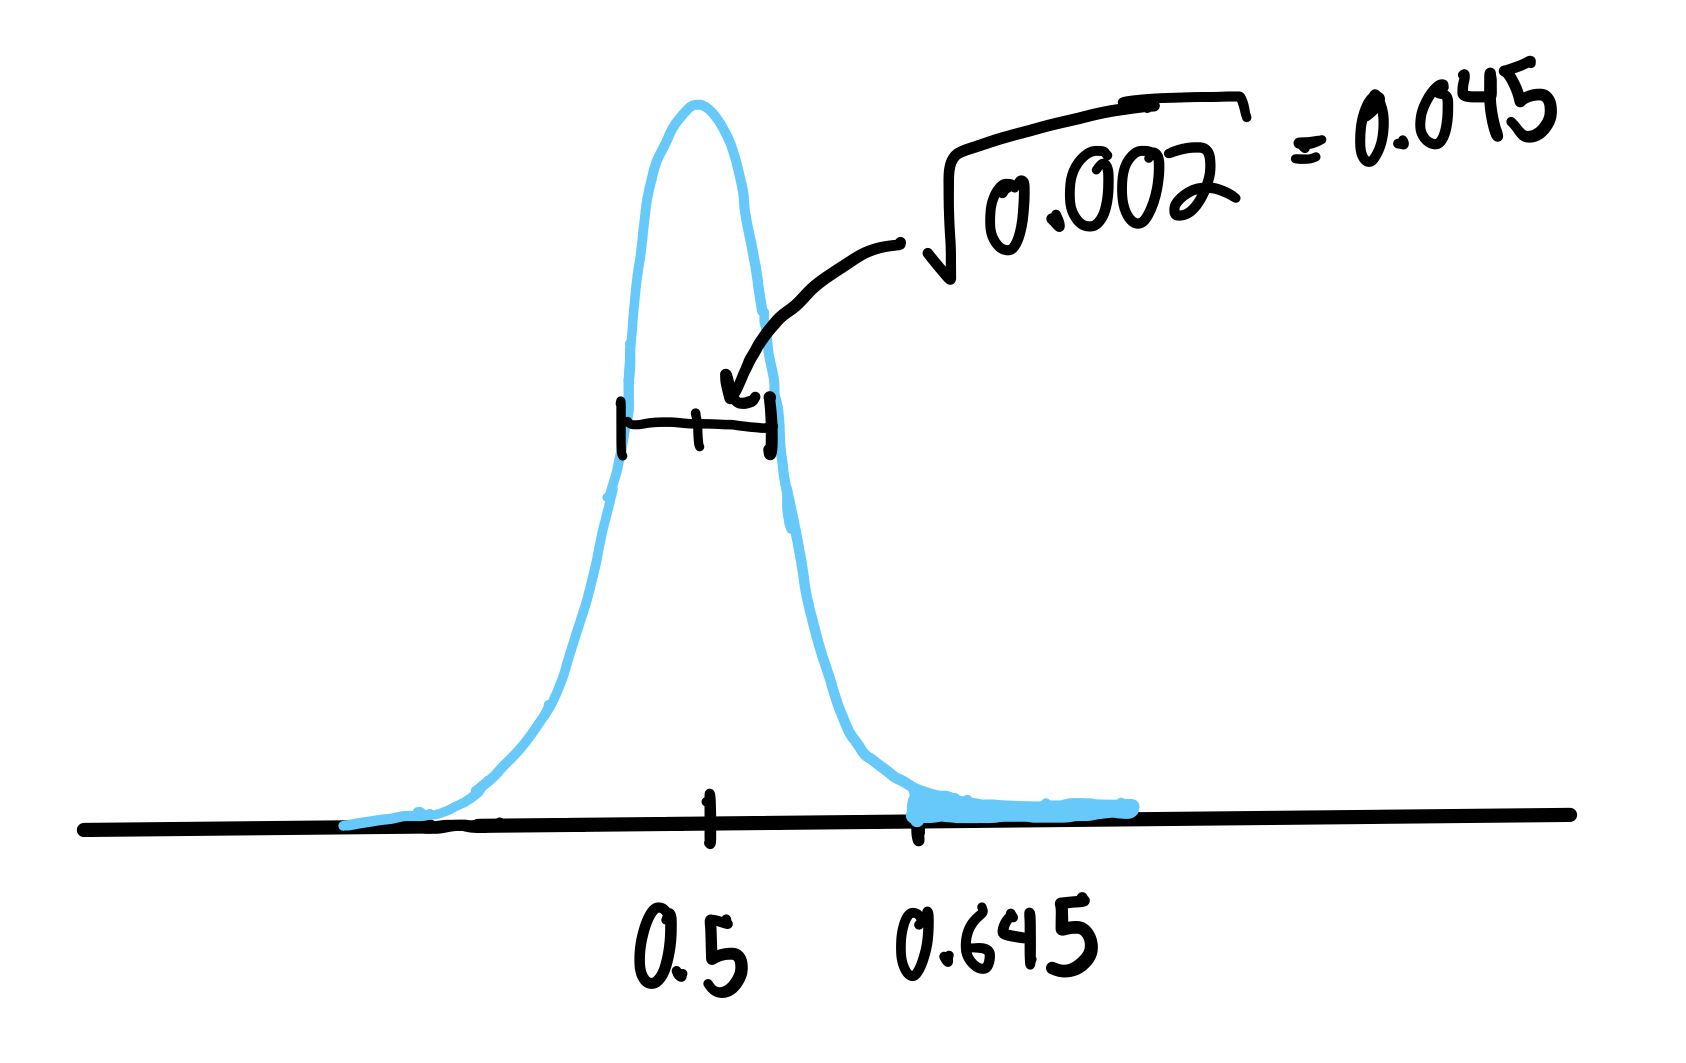
\includegraphics[scale=0.1]{figures/density.png}
\end{figure}

We compute:
\[
\mathbb P(\bar X_n \geq 0.645) \approx \mathbb P(\mathcal N(0.5, 0.002) \geq 0.645) \approx 0.003.
\]

This is our p-value. Since it's very small, we can confidently reject the null hypothesis $p = 1/2$, concluding that players do, in fact, tend to shoot to the left more often than to the right during penalty kicks.


\end{document}